\subsection{Background}
    This section focuses on the floorplan design problem of VLSI circuits by using a Mixed Linear
    Programming approach (MILP). To implement our model we used the IBM library of 
    \textit{ILOG cplex}. More precisly we choosed to implement the model by using the extension of
    \textit{DOcplex} python modeling API, \textit{Decision and Optization cplex}, which is a 
    library composed of two modules:
    \begin{itemize}
        \item Mathematical Programming Modeling for Python using \textit{docplex.mp}
              (\textit{DOcplex.MP}), which is the module we used.
        \item Constraint Programming Modeling for Python using \textit{docplex.cp} (\textit{DOcplex.CP})
    \end{itemize}

% % % % % % % % % % % % % % % % % % % % % % % % % % % % % % % % % % % % % % % % % % % % % % % % % %
\subsection{Notation}
    A new parameter will be considered in the following solution in order to correct define our model:
    \begin{align*}
        M\        &\ =\ \text{A very large positive number} > \max (width, max\_makespan)
    \end{align*}

    Next, we need to add to the variables defined in Section \ref{sec:shared_variables} the following:
    \begin{align*}
        % makespan\   &\ =\ \text{height of the plate  } i                                          \\
        % x_i\    &\ =\ \text{horizontal coordinate of bottom left corner of circuit  } i           \\
        % y_i\    &\ =\ \text{vertical coordinate of bottom left corner of of circuit  } i          \\
        u_i\    &\ =\ \begin{cases}
                              1 & \text{if circuit } i \text{ is rotated}                           \\
                              0 & \text{otherwise}
                          \end{cases}                                                               \\
        l_{i,j} &\ =\ \begin{cases}
                              1 & \text{if circuit } i \text{ is on the left side of the circuit} j \\
                              0 & \text{otherwise}
                          \end{cases}                                                               \\
        r_{i,j} &\ =\ \begin{cases}
                            1 & \text{if circuit } i \text{ is on the right side of the circuit} j  \\
                            0 & \text{otherwise}
                        \end{cases}                                                                 \\
        a_{i,j} &\ =\ \begin{cases}
                            1 & \text{if circuit } i \text{ is above the circuit} j                 \\
                            0 & \text{otherwise}
                        \end{cases}                                                                 \\
        b_{i,j} &\ =\ \begin{cases}
                            1 & \text{if circuit } i \text{ is below the circuit} j                 \\
                            0 & \text{otherwise}
                        \end{cases}
    \end{align*}

    Moreover, for what concerns the rotation model, we decide to implement a similar procedure to the
    other previously seen approaches. We implemented a couple of functions which have the scope of 
    managing the rotation and the true dimension of each circuit \(i\) according to the value of its 
    specific variable rotation \(u_i\):
    \begin{subequations}
        \label{ilp:f_dims}
        \begin{align}
            f_h(u_i) &\ = w_i \ u_i + h_i \ (1 - u_i)\\
            f_w(u_i) &\ = h_i \ u_i + w_i \ (1 - u_i)
        \end{align}    
    \end{subequations}
    Please notice that the use of such a function will not remove the linearity of each constraint,
    but it is just a name we gave to increase the readability of the report. 
% % % % % % % % % % % % % % % % % % % % % % % % % % % % % % % % % % % % % % % % % % % % % % % % % %
\subsection{Model Formalisation}
    In the following we are going to present the model formalisation for the VLSI problem as a 
    MILP, by considering the notation previously cited. Let's start with the base model without
    the rotations.
\begin{subequations}
    \label{ilp:base}
    \begin{align}
        \label{ilp:base_obj} \text{minimize}\ makespan                                   &\  &\                       \\
        \label{ilp:base_ycons}  y_c + h_c            &\ \leq\ makespan                       &\ \forall c \in C       \\
        \label{ilp:base_diffn1} x_{c_1} - x_{c_2}    &\ \geq\ w_{c_2} - M\ (1 - l_{c_1c_2})  &\ \forall c_1, c_2 \in C\\ 
        \label{ilp:base_diffn2} x_{c_1} - x_{c_2}    &\ \geq\ w_{c_2} - M\ (1 - r_{c_1c_2})  &\ \forall c_1, c_2 \in C\\
        \label{ilp:base_diffn3} y_{c_1} - y_{c_2}    &\ \geq\ h_{c_2} - M\ (1 - a_{c_1c_2})  &\ \forall c_1, c_2 \in C\\ 
        \label{ilp:base_diffn4} y_{c_1} - y_{c_2}    &\ \geq\ h_{c_2} - M\ (1 - b_{c_1c_2})  &\ \forall c_1, c_2 \in C\\
        \label{ilp:base_diffn5} l_{c_1c_2} + r_{c_1c_2} + a_{c_1c_2} + b_{c_1c_2}  &\ \geq 1 &\ \forall c_1, c_2 \in C\\
        \label{ilp:base_diffn6} l_{c_1c_2} + r_{c_1c_2} + a_{c_1c_2} + b_{c_1c_2}  &\ \leq 2 &\ \forall c_1, c_2 \in C\\
        \label{ilp:base_b_x} 0                       &\ \leq\ x_c \leq\ width - w_c          &\ \forall c \in C       \\
        \label{ilp:base_b_y} 0                       &\ \leq\ y_c \leq\ max\_makespan-h_c    &\ \forall c \in C       \\
        \label{ilp:base_b_makspan} min\_makespan     &\ \leq\ makespan \leq\ max\_makespan   &\ \forall c \in C       \\
        \label{ilp:base_b_a} 0\                      &\ \leq\ a_{c_1c_2}\ \leq\ 1            &\ \forall c_1,c_2 \in C \\
        \label{ilp:base_b_b} 0\                      &\ \leq\ b_{c_1c_2}\ \leq\ 1            &\ \forall c_1,c_2 \in C \\
        \label{ilp:base_b_r} 0\                      &\ \leq\ r_{c_1c_2}\ \leq\ 1            &\ \forall c_1,c_2 \in C \\
        \label{ilp:base_b_l} 0\                      &\ \leq\ l_{c_1c_2}\ \leq\ 1            &\ \forall c_1,c_2 \in C
    \end{align}    
\end{subequations}
    
    Also for what concerns ILP, the VLSI problem had been defined with the objective of minimizing 
    the chip height. This can be seen in the model in the equation \ref{ilp:base_obj} where it is
    shown the problem direction, namely the minimization of the integer variable \(makespan\).
    In order to complete the project task, it is necessary to minimize the variable \(makespan\) which
    is an integer variable with lower bound \(min\_makespan\) and with upper bound \(max\_makespan\).
    Please notice also that the boundaries \(min\_makespan\) and \(max\_makespan\) had been computed
    in the same way as for the previous approaches (i.e. SAT, CP and SMT).\\

    For what concerns the constraints, the first one to analyse is the one that constraints
    (equation \ref{ilp:base_ycons}) the variable \(y\) to place blocks for which vertical dimension
    doesn't exceed the value associated with the variable \(makespan\).\\

    Now the foucus should be posed on the constraints \ref{ilp:base_diffn1}-\ref{ilp:base_diffn6}.
    These constraints achieve the same task as the \textit{diffn} constraint in CP. More in
    detail, we implemented this constraint in ILP by imposing a set of equations. As we know
    it is defined in CP as \ref{eq:diffn}. So, in order to have the same result of the disjoint
    clause conditions, we need to control the variable's results. The constraints 
    \ref{ilp:base_diffn1}-\ref{ilp:base_diffn4} states the position of a circuit \(c_1\) respect to
    another circuit \(c_2\). The auxiliary parameter \(M\) has the scope to falsify the equations 
    \ref{ilp:base_diffn1}-\ref{ilp:base_diffn4}
    when the correspondent variable is set to 0. Please notice that \(M\) is a parameter that can
    be set by the user, we just want to highlight the fact that for its nature \(M\) is constrained
    to be higher than the difference between any couple of \(x\) variables and any couple of \(y\)
    variables, so we decided to set it:
    \begin{align*}
        M\ =\ \max{max\_makespan, width} + 1 
    \end{align*}
    We used for our implementation the smaller value Then the subsequent constraints 
    \ref{ilp:base_diffn5}-\ref{ilp:base_diffn6} are needed to allow the sum of the binary variables 
    (namely \(r_{c_1c_2}\), \(l_{c_1c_2}\), \(a_{c_1c_2}\) and \(b_{c_1c_2}\)) belonging in in the range
    between \(1\) and \(2\). \\
    
    Finally, the last ones are just bounding constraints, which describe the upper and lower bounds
    of the variables. More in details, while the integer variables \(x_c\) can be in the range 
    between \(0\) and \(width-w_c\) (see constraint \ref{ilp:base_b_x}), the variables \(y_c\) 
    can have values in the range between \(0\) and \(makespan-h_c\) (see constraint 
    \ref{ilp:base_b_y}). This is due to the fact that we cannot place boxes in a position such that 
    the chip's dimension exceeds the circuit plate both in high and in width. Then, since all the 
    variables of the constraints \textit{diffn} are binary, their value should fall in the range 
    \(0\) and \(1\).
% % % % % % % % % % % % % % % % % % % % % % % % % % % % % % % % % % % % % % % % % % % % % % % % % %

\subsection{Rotation}
    The next step consists to extend the model in order to take into account also the box rotation.
    For this scope, we introduced, as we did also in the previous sections, a new set of binary 
    variables \(u_c\). 

    \begin{subequations}
        \label{ilp:rot}
        \begin{align}
        \label{ilp:rot_obj} \text{minimize}\ makespan                                   &\  &\                       \\
        \label{ilp:rot_ycons}  y_c + f_h(u_c)       &\ \leq\ makespan                       &\ \forall c \in C       \\
        \label{ilp:rot_diffn1} x_{c_1} - x_{c_2} &\ \geq\ f_w(u_{c_2}) - M\ (1-l_{c_1c_2})  &\ \forall c_1, c_2 \in C\\ 
        \label{ilp:rot_diffn2} x_{c_1} - x_{c_2} &\ \geq\ f_w(u_{c_2}) - M\ (1-r_{c_1c_2})  &\ \forall c_1, c_2 \in C\\ 
        \label{ilp:rot_diffn3} y_{c_1} - y_{c_2} &\ \geq\ f_h(u_{c_2}) - M\ (1-a_{c_1c_2})  &\ \forall c_1, c_2 \in C\\ 
        \label{ilp:rot_diffn4} y_{c_1} - y_{c_2} &\ \geq\ f_h(u_{c_2}) - M\ (1-b_{c_1c_2})  &\ \forall c_1, c_2 \in C\\ 
        \label{ilp:rot_diffn5} l_{c_1c_2} + r_{c_1c_2} + a_{c_1c_2} + b_{c_1c_2}  &\ \geq 1 &\ \forall c_1, c_2 \in C\\
        \label{ilp:rot_diffn6} l_{c_1c_2} + r_{c_1c_2} + a_{c_1c_2} + b_{c_1c_2}  &\ \leq 2 &\ \forall c_1, c_2 \in C\\
        \label{ilp:rot_b_x} 0                       &\ \leq\ x_c \leq\ width - w_c          &\ \forall c \in C       \\
        \label{ilp:rot_b_y} 0                    &\ \leq\ y_c \leq\ max\_makespan-f_h(u_c)  &\ \forall c \in C       \\
        \label{ilp:rot_b_makspan} min\_makespan     &\ \leq\ makespan \leq\ max\_makespan   &\ \forall c \in C       \\
        \label{ilp:rot_b_a} 0\                      &\ \leq\ a_{c_1c_2}\ \leq\ 1            &\ \forall c_1,c_2 \in C \\
        \label{ilp:rot_b_b} 0\                      &\ \leq\ b_{c_1c_2}\ \leq\ 1            &\ \forall c_1,c_2 \in C \\
        \label{ilp:rot_b_r} 0\                      &\ \leq\ r_{c_1c_2}\ \leq\ 1            &\ \forall c_1,c_2 \in C \\
        \label{ilp:rot_b_l} 0\                      &\ \leq\ l_{c_1c_2}\ \leq\ 1            &\ \forall c_1,c_2 \in C \\
        \label{ilp:rot_b_u} 0\                      &\ \leq\ u_{c_1c_2}\ \leq\ 1            &\ \forall c_1,c_2 \in C
        \end{align}    
    \end{subequations}

    As we previously said, the use of the functions defined in the equation \ref{ilp:f_dims}, is 
    needed to express the correct dimension to the model to each box in each condition. In this way,
    it is possible to extend the model in a way that it can be possible to preserve the 
    formalisation of the no rotations model, i.e. the base one (see equations \ref{ilp:base}).
    Indeed, looking at the model, we didn't any changes to the objective function. We just modified
    the constraints \ref{ilp:rot_diffn1}-\ref{ilp:rot_diffn4}, so that they take into account the 
    correct dimensions and similarly the constraints \ref{ilp:rot_ycons} and \ref{ilp:rot_b_y}.

% % % % % % % % % % % % % % % % % % % % % % % % % % % % % % % % % % % % % % % % % % % % % % % % % %

\subsection{Results}
    All the experiments for the MILP technology have been executed on a laptop computer running 
    Windows 10 Pro, 64-bit, equipped with the following hardware:
    \texttt{Intel(R) Core(TM) i7-10510U CPU @ 1.80GHz, 4 cores, 16Gb Ram 2.30GHz}.\\

    As we can see in Figure \ref{fig:ILP_results1}, we obtained quite good results for the 
    first 20 instances in the model \(base\). In particular, we can notice that the time spent for
    proving the optimal solution is for the first 11 instances always less than 1 second. Things 
    start to get worse after the 17th instance when the time spent reached suddenly the
    threshold of 60 seconds. In later instances (Figure \ref{fig:ILP_results1}), things get even 
    more difficult. The tests we did shows that many instances had been jumped due to the 
    complexity of the problem, showing moreover an instability in for what concerns the time used 
    for solve the problem. \\
    
    In the case of \(rotations\) the Figure \ref{fig:ILP_results1} shows a similarity across the
    two models, it seems like the complexity of the problem didn't exceed the one of \(base\)
    until the 15th instance. Indeed, the subsequent ones appeared to be more difficult for the
    solver which failed to prove the optimality many times (look at Figure \ref{fig:ILP_results1} 
    for more details). \\ 

    \begin{figure}[H]
      \centering
      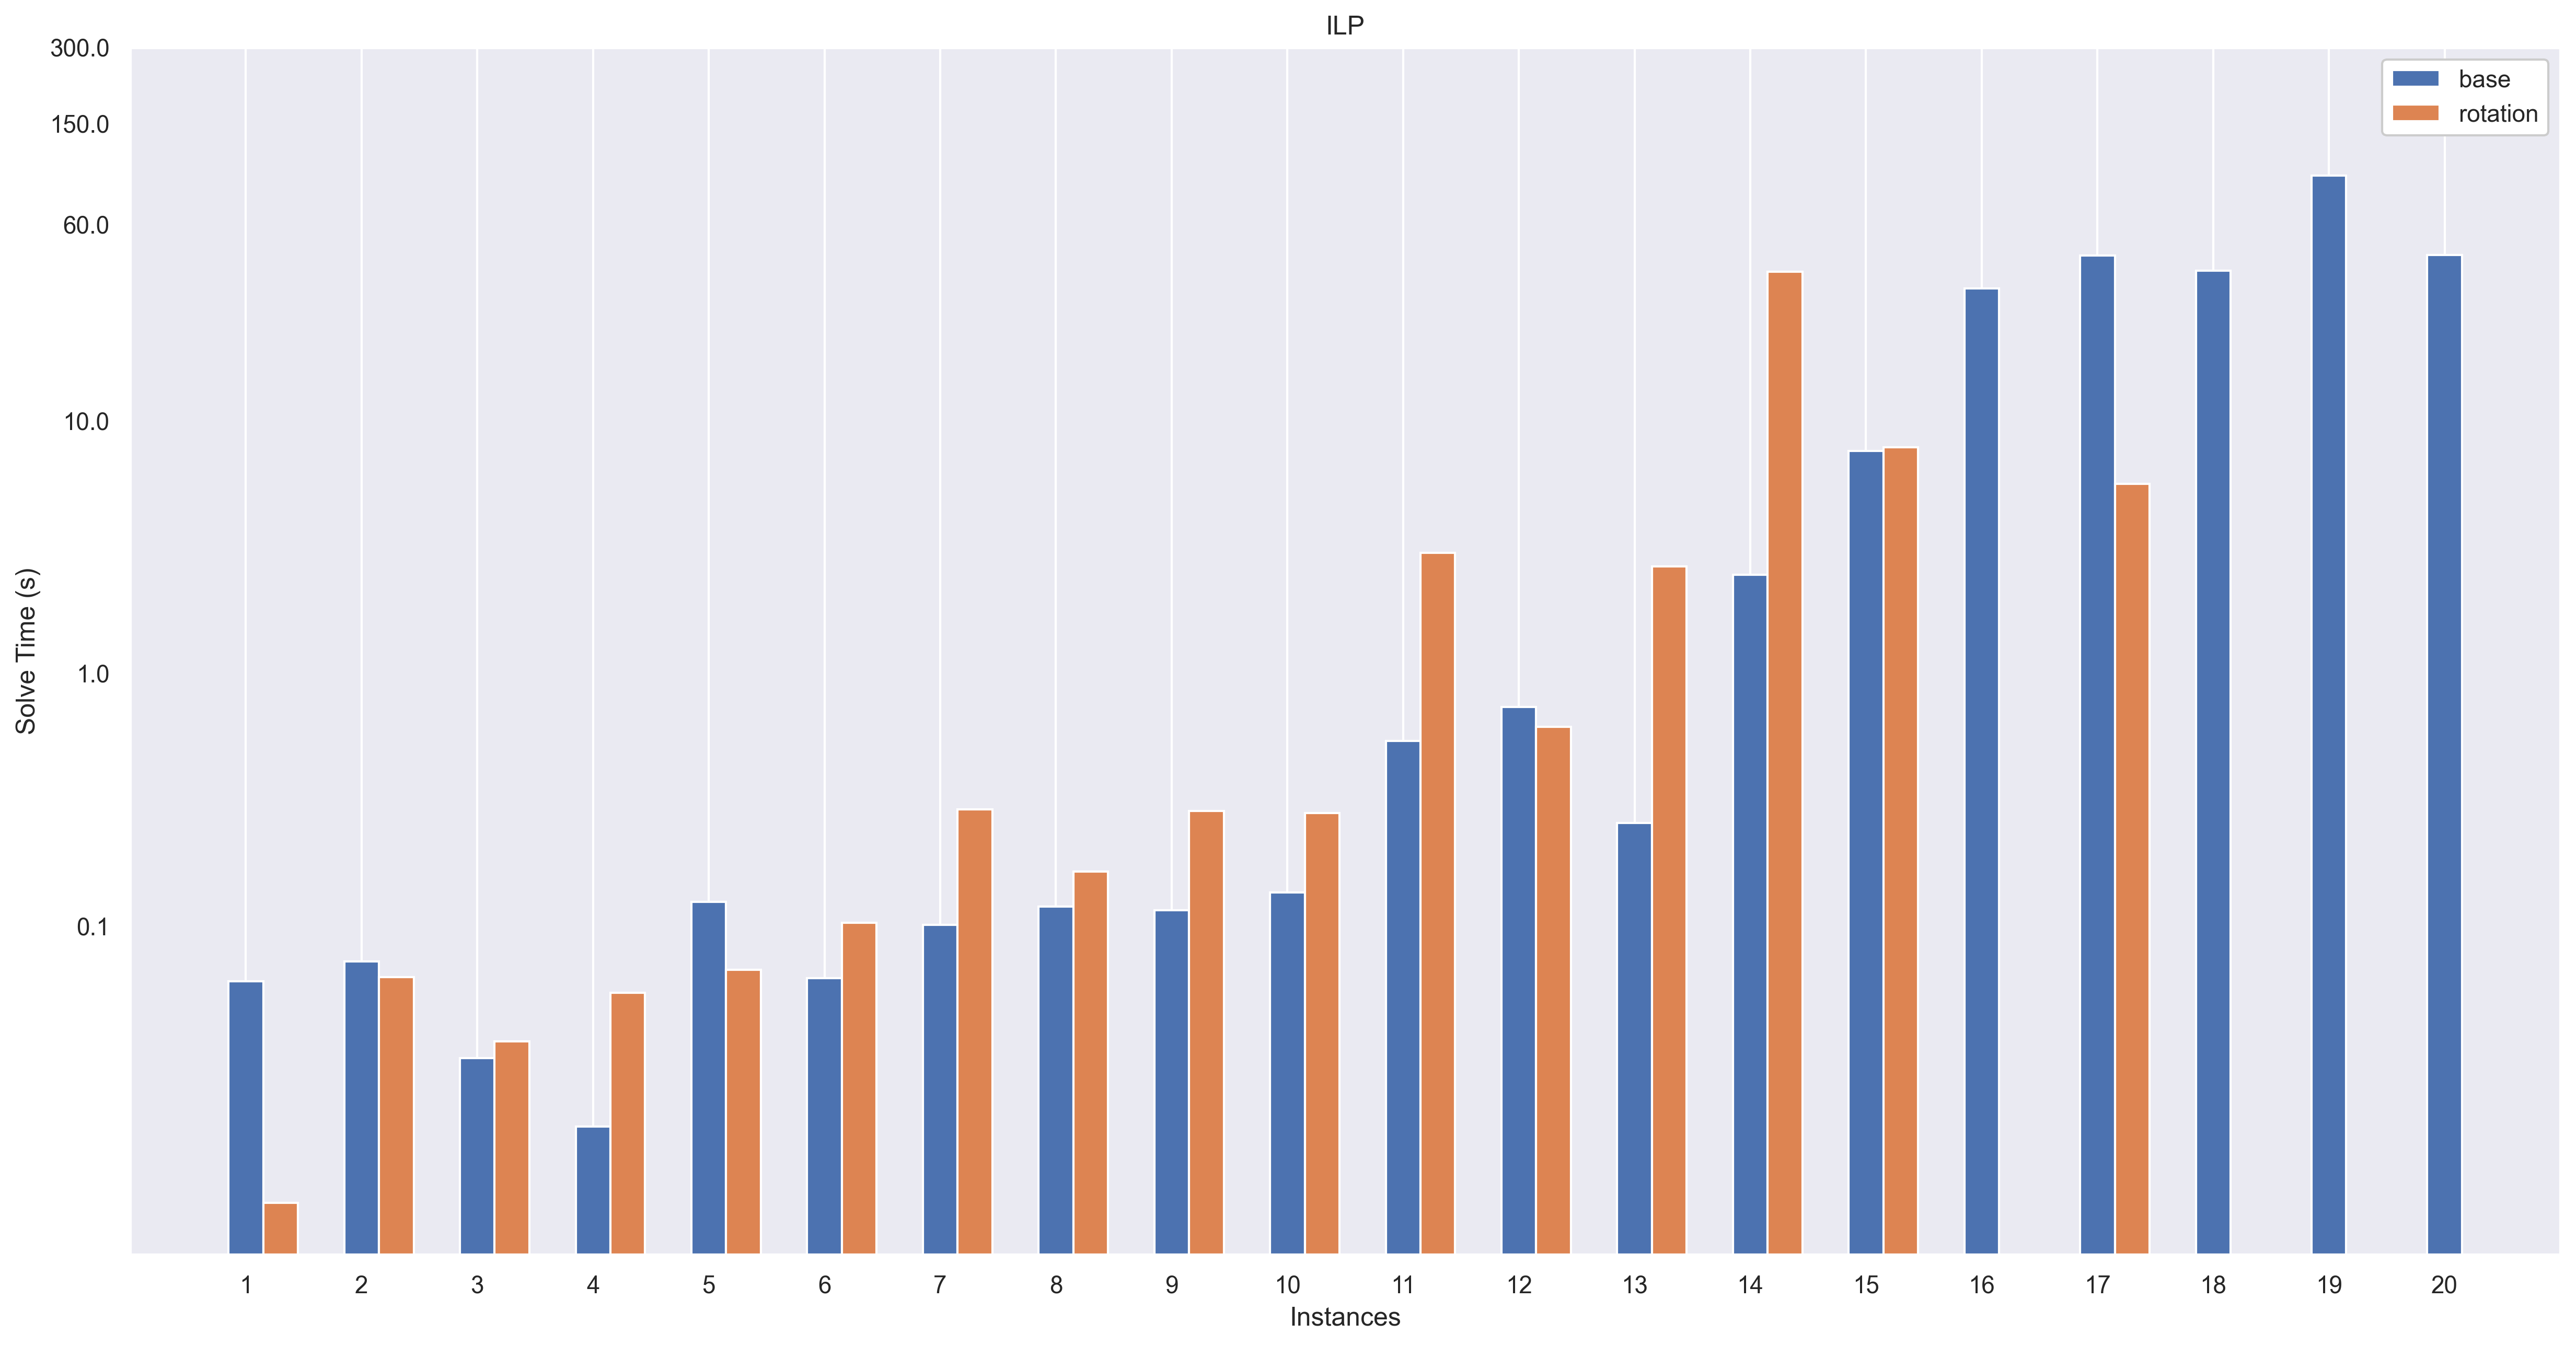
\includegraphics[width=1\textwidth]{06/results1.png}
      \caption{ILP: 
        First 20 instances total time spent for proving optimality ILP cplex solver. Quite good 
        results obtained in the fist attempt, with a progressive decrease in the quality of the 
        results as the difficulty of the problem increases.
      }
      \label{fig:ILP_results1}
    \end{figure}
    \begin{figure}[H]
      \centering
      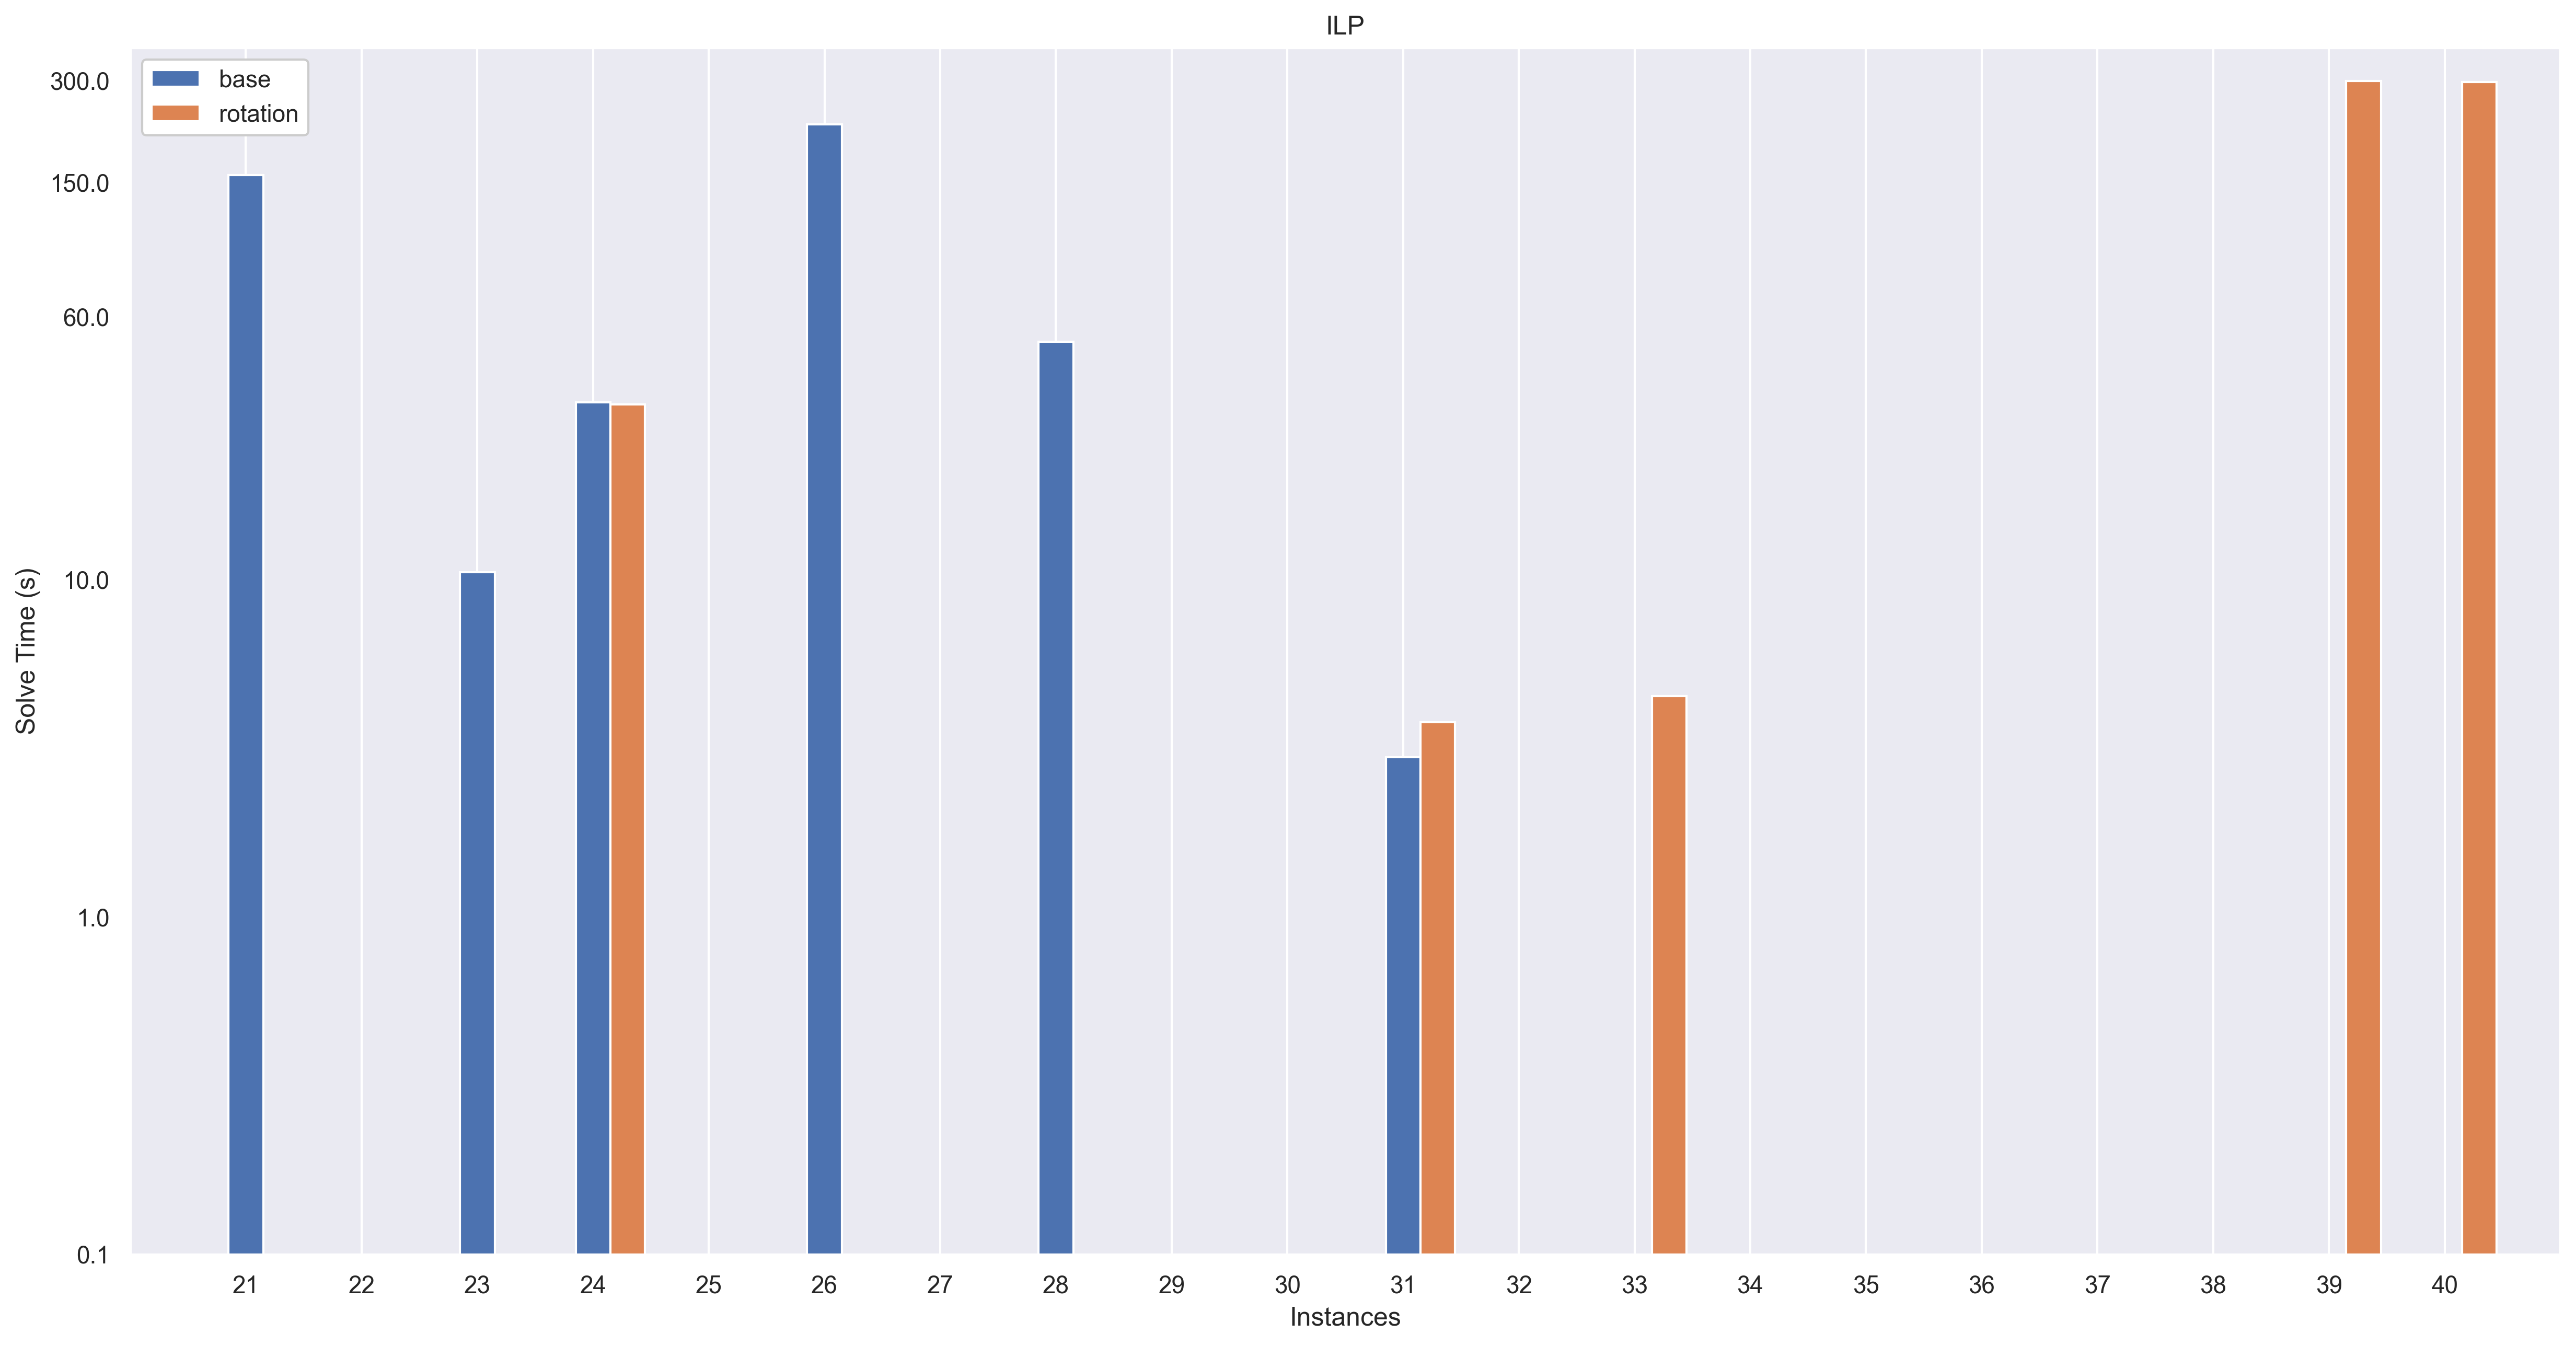
\includegraphics[width=1\textwidth]{06/results2.png}
      \caption{ILP: 
        Last 20 instances total time spent for proving optimality ILP cplex solver. Many 
        instances failed to reach the optimality with a with greater difficulty in the case of 
        \(rotation\), as it was easy to expect.
      }
      \label{fig:ILP_results2}
    \end{figure}
